\chapter{Einleitung}
\label{chap:introduction}

%%%%%%%%%%%%%%%%%%%%%%%%%%%%%%%%%%%%%%%%%%%%%%%%%%%%%%%%%%%%
\section{Motivation}
\label{sec:introduction:motivation}
%%%%%%%%%%%%%%%%%%%%%%%%%%%%%%%%%%%%%%%%%%%%%%%%%%%%%%%%%%%%

Die GPS-Navigation ist seit Jahren aus keinem Auto mehr wegzudenken. Wo früher Karten genutzt wurden und nach Straßennamen geschaut wurde, wird heute die Zieladresse in das Navigationssystem eingegeben und das System bestimmt selbstständig die aktuelle Position, die Zielposition und errechnet die bestmögliche Route.
Ein Problem der GPS-Navigation ist jedoch, dass diese nur unter freiem Himmel akzeptabel funktioniert.
Da wir uns in der Realität jedoch den Großteil unserer Zeit in Gebäuden aufhalten, ist der GPS-Ansatz dort wenig hilfreich.

Daher ist es sinnvoll, eine Alternative zu GPS zu schaffen, welche diese Navigationsfunktionen in Innenräumen ermöglicht.
Da man jedoch für Innenräume kein eigenes Navigationssystem kaufen möchte, liegt die Idee nah, dieses Konzept auf einem Gerät zu realisieren, welches viele Menschen schon besitzen und bereits für die GPS-Navigation nutzen. 
Das Smartphone.

In Abbildung 1 ist zu erkennen, wie stark die Verbreitung der Smarthphones in den letzten Jahren zugenommen hat. Dadurch kann man annehmen, dass ein Großteil der potentiellen Nutzer der Indoor Positionierung ein Smartphone besitzen.
\begin{figure}[htb]
	\centering
		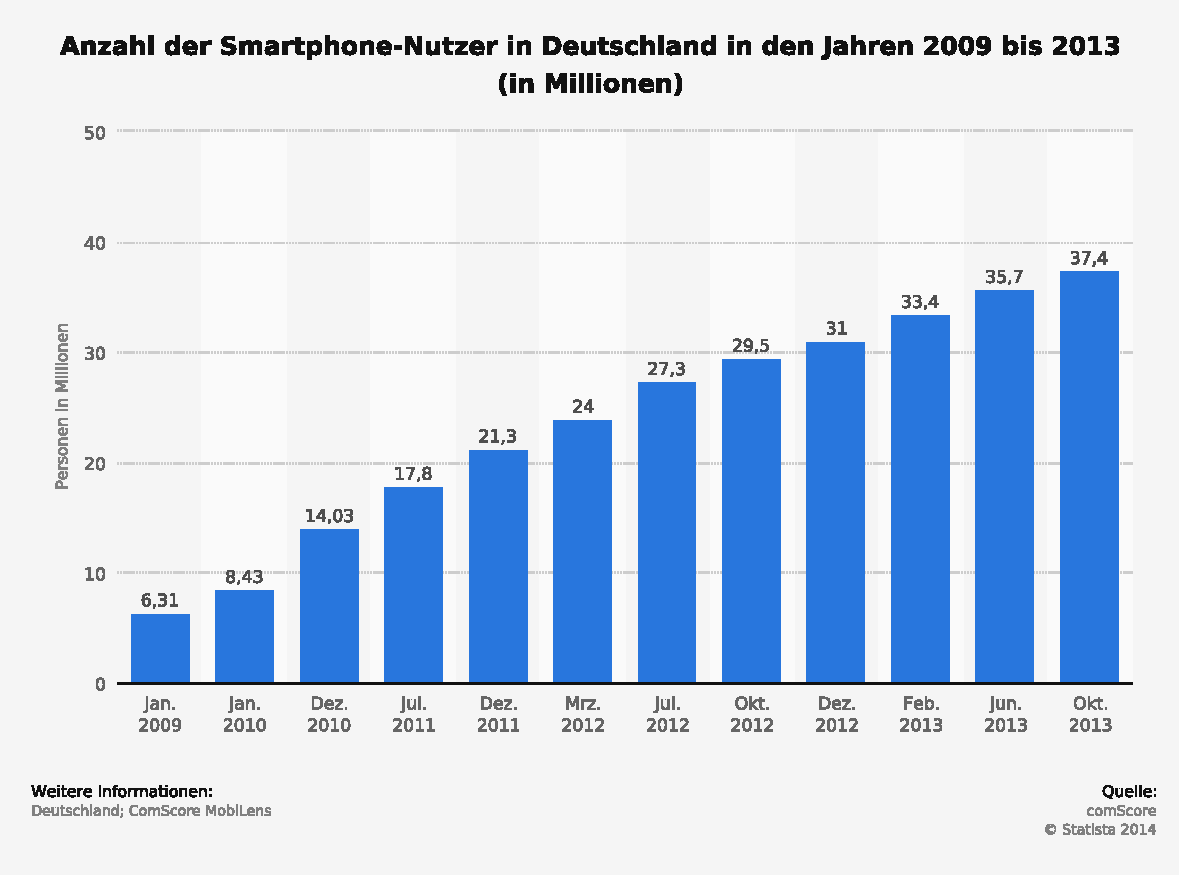
\includegraphics[height=9cm]{pictures/smartphones-germany}
		\caption{Smartphone-Nutzer in Deutschland \cite{statistic-smartphones}}
\end{figure}

Für die Realisierung der Indoor Positionierung kommen verschiedene Technologien in Frage. Darunter zum Beispiel Wireless LAN, RFID oder Bluetooth \cite{positioningOverview}.
Diese Technologien bieten sich an, da sie standardmäßig in vielen Smartphones integriert sind und so eine Nutzung des Systems ohne weitere Kosten, zum Beispiel durch Neuanschaffungen, möglich ist.

Es gibt bereits existierende Indoor Navigations-Lösungen auf dem Markt, zum Beispiel von \emph{AlterGeo} oder \emph{Skyhook Wireless}, welche jedoch auf Wireless LAN basieren. Dies bringt jedoch einige Nachteile mit sich, wie zum Beispiel die Erfordernis eines festen Stromanschlusses. Außerdem sind die bisherigen System nicht sehr genau, so gibt \emph{AlterGeo} eine Genauigkeit von 20-30 Meter an, was den Ansprüchen der Indoor Positionierung nicht gerecht wird.

Die Wahl der zu verwendenden Technologie fiel auf Bluetooth, da es die höchste Verbreitung bietet und zudem weitere Vorteile mit sich bringt. Zum einen ermöglicht Bluetooth eine schnelle und einfache Einrichtung und zum anderen benötigen die Bluetooth-Sendestationen wenig Energie, sodass nicht zwingend einen Stromanschluss vorhanden sein muss, sondern auch einen Batteriebetrieb über mehrere Monate bis Jahre hinweg möglich ist.
Außerdem bietet Bluetooth eine gute Signalreichweite, wodurch eine großflächige Abdeckung mittels weniger Sendestationen möglich ist.

Die Positionierung in Innenräumen mittels Bluetooth ist ein relativ neuer Ansatz, welcher jedoch seit der Präsentation von Bluetooth Low Energy und der Vorstellung der iBeacons-Technologie von Apple immer mehr an Aufmerksamkeit gewonnen hat. So setzt zum Beispiel Apple selbst die iBeacons-Technologie in ihren Geschäften ein, um dem Kunden gezielte Werbung zu den in der Nähe befindlichen Produkten bereitzustellen. Auch andere Unternehmen haben das Potenzial von iBeacons und Bluetooth erkannt und arbeiten an verschiedenen Einsatzmöglichkeiten für diese Technologie.

%%%%%%%%%%%%%%%%%%%%%%%%%%%%%%%%%%%%%%%%%%%%%%%%%%%%%%%%%%%%
\section{Ziele der Bachelorarbeit}
\label{sec:introduction:goal}
%%%%%%%%%%%%%%%%%%%%%%%%%%%%%%%%%%%%%%%%%%%%%%%%%%%%%%%%%%%%

Das Hauptziel dieser Arbeit ist es zu untersuchen, in wie weit sich Bluetooth Low Energy, beziehungsweise die darauf basierende iBeacons-Technologie, für eine akzeptable Indoor Positionierung eignet, um Endgeräte, zum Beispiel in Verkaufsräumen, zu orten und zu identifizieren.

Dabei soll bestimmt werden, welches Verfahren sich am Besten für die Positionierung in Innenräumen eignet und ob mit der zur Verfügung stehenden Hardware eine ausreichend genaue Positionsbestimmung realisiert werden kann. Außerdem soll die Vergleichbarkeit der Messungen zwischen verschiedenen Endgeräten untersucht werden, wobei festgestellt werden soll, ob die gemessenen Werte zwischen den Geräten übertragbar sind.

Für diese Tests werden eingangs ausschließlich Apple-Geräte genutzt, da hier eine übersichtlichere Auswahl auf dem Markt herrscht, sodass die Basis der zu nutzenden Geräte überschaubar bleibt und nur wenige Geräte getestet werden müssen. Ein weiterer Grund dafür ist, dass iOS, das Betriebssystem des Apple iPhone und iPad, bisher das einzige mobile Betriebssystem ist, welches die iBeacons-Technologie offiziell und nativ unterstützt.

Im Laufe der Bachelorarbeit soll deshalb eine iOS-Applikation entwickelt werden, welche eine Positionierung in einem Innenraum implementiert. Dabei wird das von Apple bereitgestellte CoreLocation-Framework genutzt, welches die Verarbeitung der iBeacon-Daten übernimmt. Die genutzten iBeacon-Sender kommen von Drittherstellern und befinden sich derzeit noch in einem Vorserienstadium. 

Zum Abschluss soll eine grundlegende Positionierung, eine Anzeige der aktuellen Position auf einer Karte und das Auslösen bestimmter Aktionen an festgelegten Orten implementiert sein.


%%%%%%%%%%%%%%%%%%%%%%%%%%%%%%%%%%%%%%%%%%%%%%%%%%%%%%%%%%%%
\section{Überblick}
\label{sec:introduction:overview}
%%%%%%%%%%%%%%%%%%%%%%%%%%%%%%%%%%%%%%%%%%%%%%%%%%%%%%%%%%%%
Zu Beginn der Arbeit wird ein Überblick über die verwendeten Hardware- und Softwaretechnologien, welche zur Umsetzung der Indoor Positionierung genutzt werden, gegeben. Dabei werden besonders die zugrundeliegende Bluetooth-Technologie als auch das CoreLocation-Framework, welches für die Verarbeitung der Beacon-Daten zuständig ist, genauer betrachtet. 

Im zweiten Abschnitt werden diverse Messdaten erhoben, welche die Signalausbreitung der Bluetooth-Beacons verdeutlichen. Dabei werden unter anderem die batteriebetriebenen Beacons mit stationären Beacons verglichen. Außerdem wird untersucht in wie weit sich die Empfangsstärken zwischen verschiedenen Endgeräten unterscheiden. 

Im darauf folgenden Kapitel werden auf die verwendeten Techniken zur Positionierung erörtert. Dabei wird zuerst eine Positionierung mittels Trilateration beschrieben, welche die Position anhand von Entfernungswerten zu den Basisstationen bestimmt. Danach wird die Methode des Fingerprinting näher erläutert, welche die Positionierung mittels zuvor gesammelter Positions- und Signalstärkedaten realisiert. Dabei werden verschiedene Algorithmen zur Bestimmung der Ähnlichkeit zwischen den gesammelten Fingerprintdaten in der Datenbank und den aktuell empfangenen Signalstärkedaten beschrieben.

Im letzten Teil wird die Leistungsfähigkeit der verschiedenen Algorithmen untersucht und verglichen. Dabei werden unteranderem die Genauigkeit, als auch die Robustheit der Positionsbestimmung untersucht.

Abschließend folgt ein Fazit und ein Ausblick für die Zukunft der iBeacon-Technologie und der Indoor Positionierung.
